\section{The Consolidation--Interference Duality}
\label{sec:duality}

\begin{intuition}
\textbf{What the theorem says, without symbols.} Take a cluster of
embedded points that live on the unit sphere. Two numbers describe it:
its \emph{effective dimension} $\deff$, which measures how many truly
independent directions the cluster uses, and its \emph{mean spread}
$\dbar$, which measures how tight the cluster is. Pick a retrieval
threshold $\theta$: a query ``hits'' a representative if their cosine
exceeds $\theta$. The theorem says: if you compress the cluster to $m$
representatives and the threshold slack $\thetap = 1-\theta$ is smaller
than the cluster's spread $\dbar$, then the fraction of cluster members
whose nearest representative is outside the cap is at least
$1 - c_1\, m\, (\thetap/\dbar)^{\deff/2}$.

The exponent is the active ingredient. Whenever $\thetap < \dbar$, the
base $(\thetap/\dbar)$ is less than one, and the whole quantity shrinks
exponentially in $\deff$. That exponential is the compression tax: to
keep the identity-retrieval error below any target $\eps^\ast$, the
representative budget $m$ must grow as $(\dbar/\thetap)^{\deff/2}$, which
is astronomical for $\deff = 16$ and astronomical-squared for $\deff =
32$. The deeper message: this is not a property of any particular
summarisation algorithm. It is a property of the cluster itself. Pick a
different summariser and you move around inside the bound; you cannot
escape it.
\end{intuition}

\begin{figure}[t]
\centering
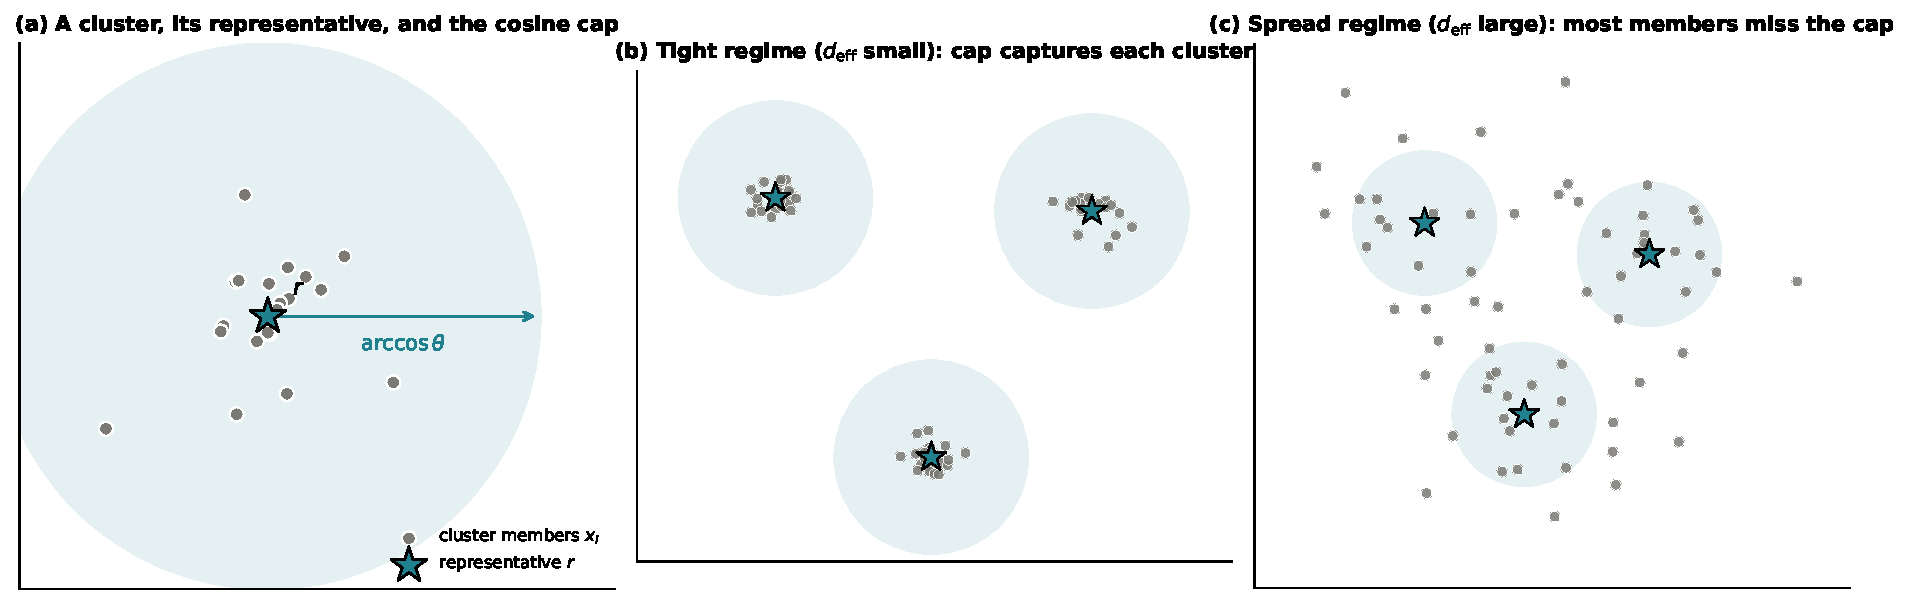
\includegraphics[width=0.98\linewidth]{figs/fig0_schematic.pdf}
\caption{\textbf{The law in one picture.} A cluster of embedded
members, a representative $r$, and a cosine cap of angular radius
$\arccos\theta$. When the cluster's effective dimension $\deff$ is
small relative to the cap (panel b), $r$ covers almost every member and
consolidation is lossless. When $\deff$ is large (panel c), most
members lie outside every cap and any single-vector summary loses
identity. The law formalises exactly when (b) holds and predicts when
(c) starts.}
\label{fig:schematic}
\end{figure}

\subsection{Setup}

Let $\clusterset = \{x_1, \ldots, x_n\} \subset \SphereD$ be a cluster on
the unit sphere. Let $\mu_\clusterset = \tfrac{1}{n} \sum_{i=1}^n
\delta_{x_i}$ be its empirical measure. The \emph{mean within-cluster
distance} is
\begin{equation}
\dbar := \frac{1}{\binom{n}{2}} \sum_{i<j}\bigl(1 - \inner{x_i}{x_j}\bigr).
\label{eq:dbar_def}
\end{equation}
A \emph{consolidator} is any map $\clusterset \mapsto \reps = \{r_1,
\ldots, r_m\} \subset \SphereD$ with $m \leq n$. For a \emph{retrieval
cap} $\theta \in (0, 1)$, the \emph{identity-retrieval error} is
\begin{equation}
\eps_{\mathrm{id}}(\clusterset, \reps) :=
\frac{1}{n} \Bigl|\Bigl\{i : \max_j \inner{x_i}{r_j} < \theta \Bigr\}\Bigr|
\;=\; 1 - \mu_\clusterset\Bigl(\bigcup_{j=1}^m H_j(\theta)\Bigr),
\label{eq:id_error_def}
\end{equation}
where $H_j(\theta) := \{x \in \SphereD : \inner{x}{r_j} \geq \theta\}$ is
the spherical cap of angular radius $\arccos\theta$ around $r_j$.
Informally, $\eps_{\mathrm{id}}$ is the fraction of source points whose
nearest representative fails to reach the cap.

\subsection{Statement}

\begin{theorem}[Consolidation--Interference Duality]
\label{thm:duality}
Let $\clusterset = \{x_1, \ldots, x_n\} \subset \SphereD$ be a cluster
with local effective dimension $\deff$ and mean within-cluster distance
$\dbar$. Let $\reps = \{r_1, \ldots, r_m\} \subset \SphereD$ be any set
of $m \leq n$ representatives produced by any consolidator. Fix a
retrieval threshold $\theta \in (0,1)$ and write $\thetap := 1 - \theta$.
If $\thetap < \dbar$, then
\begin{equation}
\eps_{\mathrm{id}}(\clusterset, \reps)
\;\geq\; 1 - c_1\, m\, \left(\frac{\thetap}{\dbar}\right)^{\deff/2},
\label{eq:duality_bound}
\end{equation}
where $c_1 > 0$ is an absolute constant, independent of $m$, $n$, $d$, and
the choice of consolidator.
\end{theorem}

The proof is a two-step cap-volume argument: a local cap-volume lemma
bounds the mass of a single cap under $\mu_\clusterset$ by $c_1
(\thetap/\dbar)^{\deff/2}$, and a union bound over the $m$ representatives
inflates that bound by a factor of $m$. The full proof is in
Methods (\S\ref{sec:methods:proof}).

\subsection{Two immediate corollaries}

\begin{corollary}[Compression lower bound]
\label{cor:compression}
Fix any target $\eps^\ast \in (0, 1)$. To achieve $\eps_{\mathrm{id}} \leq
\eps^\ast$ the consolidator must use at least
\begin{equation}
m \;\geq\; c_1^{-1}\,(1 - \eps^\ast)\,\left(\frac{\dbar}{\thetap}\right)^{\deff/2}
\label{eq:compression_bound}
\end{equation}
representatives. The representative budget grows exponentially in $\deff$,
with base $\dbar / \thetap$.
\end{corollary}

\begin{corollary}[Isotropic degeneracy]
\label{cor:iw}
On a cluster whose embedding-space second moments are isotropic,
importance-weighted consolidation (centroid with inverse-rank weights)
converges to the uniform centroid at rate $O(1/n)$ and therefore inherits
the centroid's bound with no improvement.
\end{corollary}

Corollary~\ref{cor:iw} is what makes the importance-weighted baseline
indistinguishable from centroid on every real text corpus we tested (see
\S\ref{sec:e1_validation} and \S\ref{sec:template_collapse}): real
clusters are close to isotropic in their effective subspace, so the
weighted mean collapses to the uniform mean.

\subsection{Three ways to read Equation~\eqref{eq:duality_bound}}
\label{sec:duality:readings}

Equation~\eqref{eq:duality_bound} is the same formula read in three
different directions. Each reading is useful.

\paragraph{Read 1: A floor on error.} Fix a corpus (so $\dbar$ and
$\deff$ are given) and a retrieval policy ($\theta$ given). Then the
right-hand side is a function of $m$ alone. It tells you: to keep
identity-retrieval error below $\eps^\ast$, your budget $m$ cannot
shrink below the threshold in Corollary~\ref{cor:compression}. This is
the \emph{operational} reading --- ``how small can I make my index and
still get answers back?''.

\paragraph{Read 2: A test on cluster shape.} Fix $m$ and $\theta$. Then
the right-hand side is a function of $\deff$ and $\dbar$ alone. It tells
you which kinds of clusters can be compressed aggressively (small
$\deff$, tight $\dbar$) and which cannot (large $\deff$, spread
$\dbar$). This is the \emph{diagnostic} reading --- ``does my corpus live
on the right side of the regime boundary?''.

\paragraph{Read 3: A duality.} The same spectral quantity
$(\thetap/\dbar)^{\deff/2}$ governs the No-Escape bound of the
previous paper~\cite{priceOfMeaning2026}, which says any kernel-threshold
memory with finite $\deff$ forgets by interference under retrieval
noise. Forgetting under noise and identity loss under compression are
therefore two readings of the \emph{same} inequality on the cluster's
cap-volume quantity. This is why we call the theorem a
\emph{Consolidation--Interference Duality}: it is not a new bound; it is
the No-Escape bound, specialised to the compression setting.

\subsection{What the bound does and does not promise}
\label{sec:duality:caveats}

Because we will spend a significant fraction of Section~\ref{sec:e1_validation}
measuring how well Equation~\eqref{eq:duality_bound} fits real data,
it is worth being explicit about what it is and is not.

\paragraph{It is a lower bound, not a prediction.} The theorem says
consolidation cannot do better than the right-hand side. A specific
consolidator might do much worse --- that failure is strategic rather
than geometric. The point of introducing GAC in \S\ref{sec:gac} is to
get close to the bound, not to break it.

\paragraph{It is tight only in the tight regime $\thetap < \dbar$.}
When $\thetap \geq \dbar$ the cap-volume lemma becomes vacuous: the cap
can contain the entire cluster and the bound reads
$\eps_{\mathrm{id}} \geq 1 - c_1 m \cdot 1$, which is non-trivial only
if $c_1 m < 1$. For $\thetap = \dbar$ the right-hand side sits at the
boundary of usefulness; for $\thetap > \dbar$ (retrieval cap looser than
cluster spread) the theorem stops giving information. This is the
\emph{spread regime}. Empirically (\S\ref{sec:e1_validation}) the bound
is tight enough to predict strategy rankings in the spread regime, but
not tight enough to predict absolute error values there.

\paragraph{$c_1$ is an absolute constant, but not a small one.} The proof
gives $c_1$ in terms of constants from the Berry--Esseen inequality and
an exponential correction for concentration on the sphere. We do not
optimise $c_1$ in the proof; we calibrate it empirically in
\S\ref{sec:e1_validation:calibration} and find $c_1^{95} \approx 0.05$ in
the tight regime, within an order of magnitude of the ideal Berry--Esseen
constant that the cap-volume lemma reduces to. An anisotropic refinement would produce a smaller $c_1$ at
the price of a more delicate proof; we leave that to future work.

\paragraph{Cluster-conditional, not marginal.} The effective dimension
$\deff$ and spread $\dbar$ are computed on \emph{one} cluster, not on
the ambient embedding. The paper's previous installment documented that
\emph{global} $\deff$ of production sentence encoders is $\approx
16$~\cite{geometryOfForgetting2026}; the local $\deff$ on a single
cluster of paraphrases is much smaller (we measure $\deff_{\mathrm{local}}
\in \{1.5, 2.3, 5.5, 12.6, 30.1, 107.5\}$ across our six corpora in
\S\ref{sec:template_collapse}). The bound applies cluster-by-cluster, and
the bound for the worst cluster dominates the bound for the whole
memory.

\subsection{What is proved, what is observed, what is inferred}
\label{sec:duality:proved_observed_inferred}

Before turning to experiments we separate three claim categories so
that later sections can be read precisely.

\paragraph{Proved.} For any consolidator acting on a unit-norm cluster,
in the tight regime $\thetap < \dbar$,
identity-retrieval error is lower-bounded by the right-hand side of
Equation~\eqref{eq:duality_bound} with a universal constant $c_1$ whose
value follows from the cap-volume lemma
(\S\ref{sec:methods:proof}). This is the theorem.

\paragraph{Empirically observed.} The tight/spread phase boundary at
$\dbar = \thetap$ is visible in the $400$-cell synthetic grid of
\S\ref{sec:e1_validation} and organises the ordering of six real-text
corpora and six sentence encoders of
\S\ref{sec:template_collapse}. Restricted to the tight regime, the
bound's shape (exponent $\deff/2$) is quantitatively accurate with a
calibrated $c_1^{95} \approx 0.05$ over $12{,}400$ cells. In the spread
regime, the ordering of strategies is preserved but absolute error
magnitudes are not sharply predicted by the bound.

\paragraph{Inferred.} The dominance of centroid over adaptive routing
on five real-text corpora (\S\ref{sec:gac:ablation}) is
\emph{explained by} the finding that these corpora sit in the tight
regime the theorem declares safe. The regime-dependent three-way
downstream split on Natural Questions, HotpotQA, and PopQA
(\S\ref{sec:e7}) is \emph{consistent with} the cap-coverage prediction
for which operator the law prefers on each corpus. These are
interpretive claims: the theorem does not \emph{prove} that centroid
must dominate on a given real corpus, but it predicts \emph{which
corpora should admit} centroid dominance, and that prediction holds in
the data we collected.

\paragraph{Not claimed.} The theorem is stated and proved for unit-norm
embedding clusters under cosine-threshold retrieval. We do not claim
that it applies unchanged to non-contrastive embedding spaces, to
non-unit-norm representations (e.g.\ raw LLM hidden states), to
multimodal embeddings, or to biological memory. These are settings in
which the law's structural form is a natural hypothesis to test; the
test has not yet been done.
